\section{Introduction}
Like many other scientific research fields chemistry has experienced an explosion of research over the last few decades. This ever growing corpus provides ample ground for data mining approaches to extract meaning from vast data. Large chemistry datasets have been used to generate models for molecule generation \cite{}, reaction yield prediction \cite{}, and property prediction \cite{}. Existing approaches have relied on labeled data and as a result there has been little use of the thousands of journal and conference articles. \\
While some molecules have easily recognizable names like hydrogen-peroxide ($H_20_2$) most molecules are rare enough that they do not. To solve this problem, chemists have developed a textual to represent molecules called Simplified Molecular-input Line-entry System (SMILES) \cite{}. SMILES can is a method of describing the structure of a molecule using ASCII strings and SMILES can be used to generate two and three dimensional molecular representations at scale. For example, the molecule benzene can be represented by the SMILES string  "c1ccccc1". In recent years, deep learning researchers have focused on using large corpora of SMILES \cite{} and this representation has become the backbone on which most machine learning chemistry research is performed. While SMILES is a reproducible method of representing molecules they are rarely present in chemistry literature. Instead, chemistry literature usually is focused on two dimensional images of molecules and their reactions which are created by drawing programs like ChemSketch and ChemDoodle. Without a way to decode this images the literature is essentially full of recipes written in a language we cannot understand. Since literature seldom includes textual molecule representations many chemist use the previously mentioned drawing programs to recreate the molecules and reactions. This approach is tedious, error prone, time consuming and difficult to scale which drives the need for an automated, high throughput molecular prediction system. \\
Being able to accurately extract molecules from literature is vital to any downstream tasks like question answering and information extraction. Without the proper molecules building systems that enables chemists to be more productive is difficult as answering questions about molecular properties, related compounds, and predicted outcomes will all be wrong if the molecule is wrong. Moreover, without accurate molecule extraction any method that tries to mine large corpora is likely to be unsuccessful. As a result, any improvement in the quality of molecule prediction will provide amplified gains in downstream tasks. 
While the notion of extracting molecules from literature is by no means a novel task the majority of methods rely on handcrafted rules and built on the intuitions of chemists. To extract information from chemistry literature there are essentially two main tasks: segmentation, and molecule prediction. Segmentation systems are focused on segmenting parts of the chemistry documents and inferring what the pixel coordinates of a molecule or reaction may be. Molecule prediction systems are focused on extracting the output of segmentation systems and predicting the most likely molecule for each given molecule segment found in the target document. Finding the segmentation software fairly successful our work focuses on molecule prediction. Despite no large dataset of annotations, this molecule prediction is a perfect candidate for data hungry solutions because the creation of artificial datasets is fairly easy. Software tools such as RDKIT can use SMILES strings to create molecules of varying style, shape, and size (pixels) at scale. \\
Independently of chemistry, in the last few years computer science researchers have been able to use large data regimes and neural network architecture like transformers \cite{} and convolutional networks \cite{} to build performant image captioning systems. Systems in chemistry have succesfully leverage residual network systems trained on Image-Net \cite{} to produce molecule predcition systems \cite{DE

We study approaches for parsing molecular structure as it applies to molecule prediction. 
While there do exist prio
Previous work

\begin{figure}[!htb]
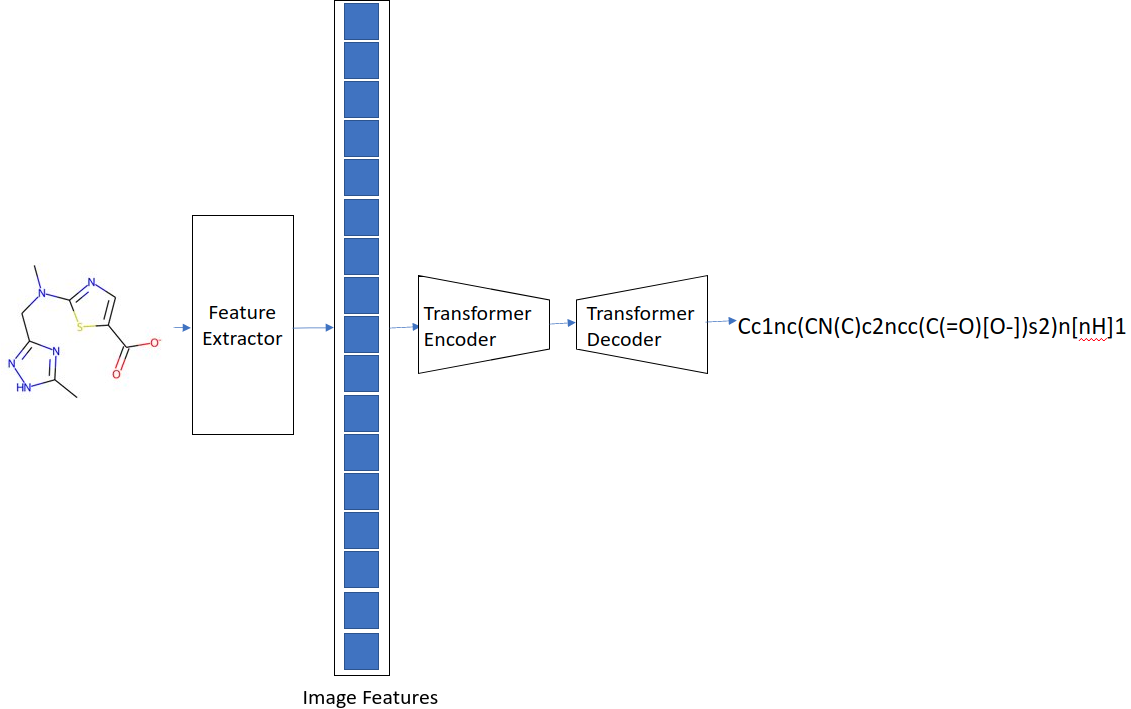
\includegraphics[height=7cm]{image/captioning-task.png}
\caption{Our image captioning system relies on a RESNET-101 based system to extract features from each molecule image followed by a transformer based encoder and decoder to produce candidate SMILES strings.}
\label{fig:system description}
\end{figure}


In summary, the main contributions of this paper are as follows:
\begin{enumerate}
    \item We introduce the IMG2SMI molecule prediction model. Using a RESNET-101 backbone and a transformer based encoder-decoder stack it produces 
    \item We introduce a novel dataset named IMG2SMI. The dataset features 80 million p
    \item We provide a through study of methods of processing SMILES strings for image captioning.
\end{enumerate}


\heng{1. define the task}
\heng{2. why the task is important: for human users to disambiguate; for downstream NLP components such as IE and QA to use}
\heng{3. limitation of previous work... did not use embedding representation etc.}
\heng{4. our novelty: we propose a 5-way translation: 2-D structure, 3-D structure, SMILES, natural language description. A novel multi-modal representation. }
